% Accuracy-vs-memory (Pareto) panels, avg-accuracy view -- one panel per pool
% size (2x DS, 2x Qwen2.5, 3x Qwen3-32B, 5x Llama, 7, 9, 12), stacked in a
% single column. Upload the figs/ directory next to this file.
%
% Requires only \usepackage{graphicx}.
%
% Sizing: each panel is 5.5in x 2.5in, so at \columnwidth (~3.33in in a
% two-column template) a panel is ~1.5in tall; all seven panels + legend are
% ~12.5in and DO NOT fit one column of one page. The two floats below split
% the stack 4 + 3 (LaTeX places them on consecutive columns/pages). In a
% single-column document (e.g. arXiv preprint) you can merge them into one
% \begin{figure}[p] and drop the second float.

\begin{figure}[t]
  \centering
  \setlength{\lineskip}{3pt}
  
\includegraphics[width=\columnwidth]{figs/pareto_legend_avg.pdf}\\
  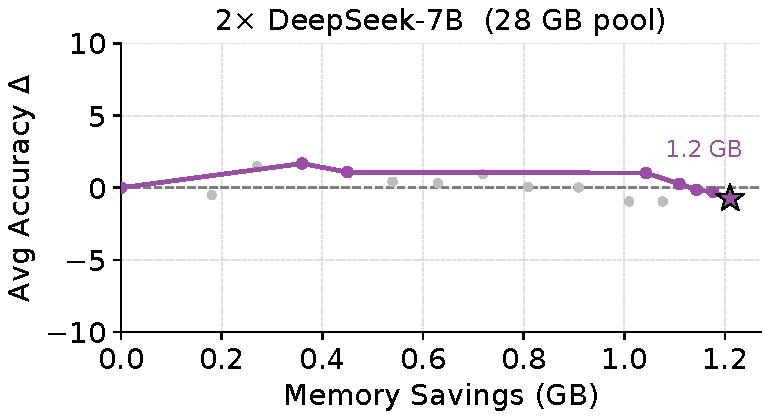
\includegraphics[width=\columnwidth]{figs/pareto_deepseek2_avg.pdf}\\
  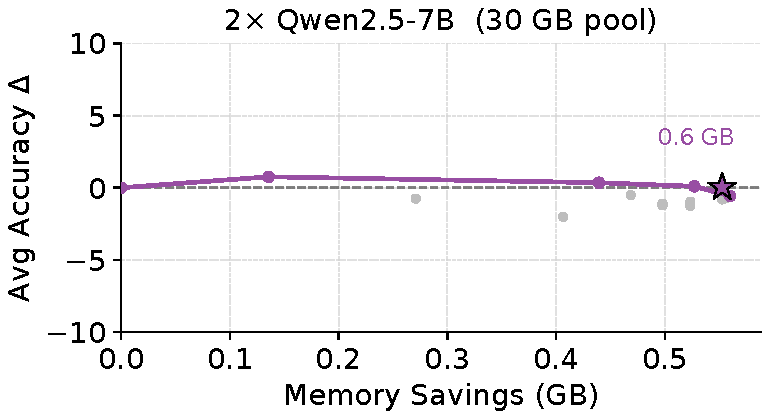
\includegraphics[width=\columnwidth]{figs/pareto_qwen25_2_avg.pdf}\\
  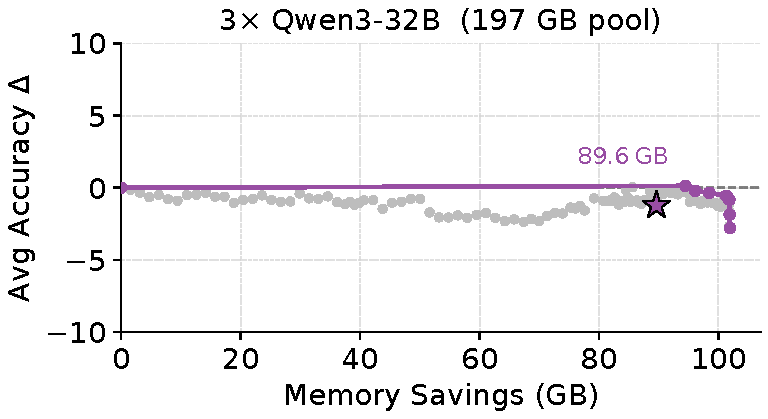
\includegraphics[width=\columnwidth]{figs/pareto_fig5a_avg.pdf}\\
  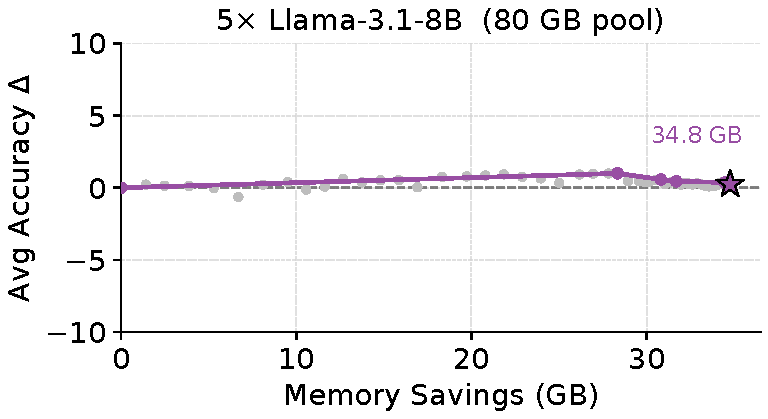
\includegraphics[width=\columnwidth]{figs/pareto_fig5b_avg.pdf}
  \caption{Accuracy--memory trade-off per model pool (average accuracy
  $\Delta$ across the pool's models; continued in
  Figure~\ref{fig:pareto-avg-2}). Grey points are explored merge
  configurations, the purple line is their Pareto frontier anchored at the
  unmerged pool, and the star is Sandhi's selected operating point, chosen so
  \emph{every} model stays within the user-set accuracy bound of its own
  unmerged baseline.}
  \label{fig:pareto-avg-1}
\end{figure}

\begin{figure}[t]
  \centering
  \setlength{\lineskip}{3pt}
  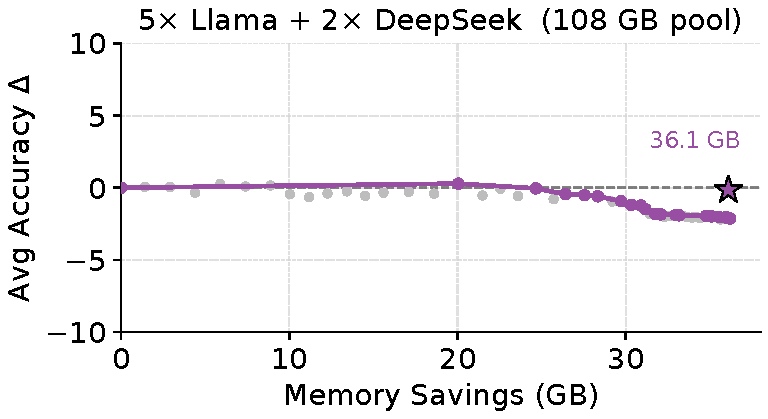
\includegraphics[width=\columnwidth]{figs/pareto_llama5_deepseek2_avg.pdf}\\
  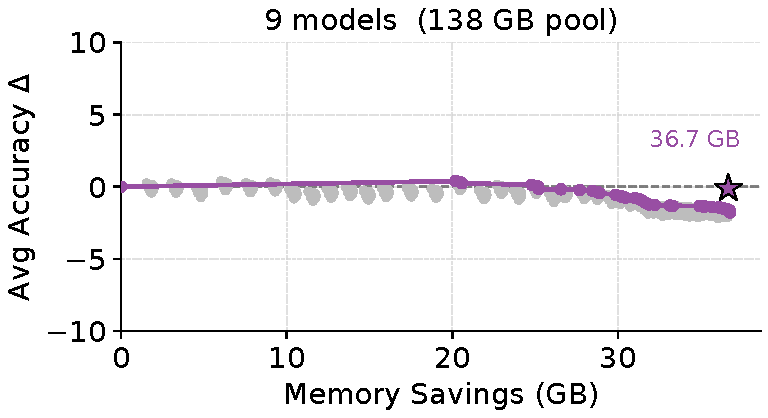
\includegraphics[width=\columnwidth]{figs/pareto_9model_avg.pdf}\\
  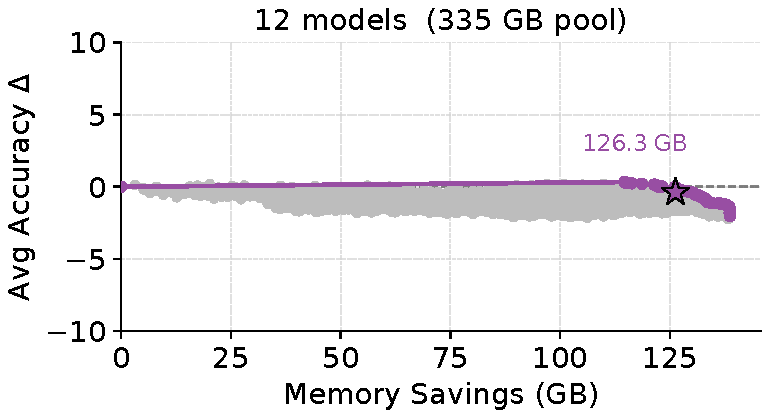
\includegraphics[width=\columnwidth]{figs/pareto_12model_avg.pdf}
  \caption{Accuracy--memory trade-off per model pool, continued from
  Figure~\ref{fig:pareto-avg-1}: the 7-, 9-, and 12-model pools. The 9- and
  12-model pools are additive compositions of the atom pools' sweeps (savings
  sum; accuracy is the model-count-weighted average), so every grey point is
  a deployable combination of per-pool configurations.}
  \label{fig:pareto-avg-2}
\end{figure}
